\noindent  Para  representar la  posición  relativa  del vehículo  con
respecto  al espacio  de  estacionamiento, se  propone  un sistema  de
coordenadas cilíndricas en el cual el origen se encuentre en la cámara
del vehículo. Esta elección provee un marco de referencia que facilita
la  medición de  las distancias  y ángulos  necesarios para  maniobrar
adecuadamente  durante   el  estacionamiento.
\noindent Utilizando coordenadas cilíndricas,  es posible describir la
posición  del  vehículo en  términos  de  distancia radial,  ángulo  y
altura, con el origen en la cámara del vehículo permite representar de
manera  directa las  relaciones  espaciales entre  el  vehículo y  los
límites  del espacio  de  estacionamiento. La  altura  conocida de  la
cámara respecto al  suelo proporciona un eje  de referencia constante,
mientras que los ejes orientados  según la dirección y lateralidad del
vehículo facilitan  la interpretación  y cálculo  de la  orientación y
desplazamiento necesarios para estacionar correctamente.

\subsection{Origen del sistema de coordenadas}
Consideramos que el origen del sistema está centrado en la cámara del vehículos, de tal manera que los ejes ortonormales del sistema se definen como sigue:
\begin{itemize}
    \item El eje $z$ se define como un vector unitario en dirección vertical  apuntando hacia el suelo.
    \item El eje $x$ se define como un vector unitario que apunta hacia el frente del vehículo.
    \item El eje $y$ se define como un vector unitario que apunta hacia el lado derecho del vehículo.
\end{itemize}

\begin{figure}[!ht]
    \centering
    \begin{subfigure}{0.4\textwidth}
        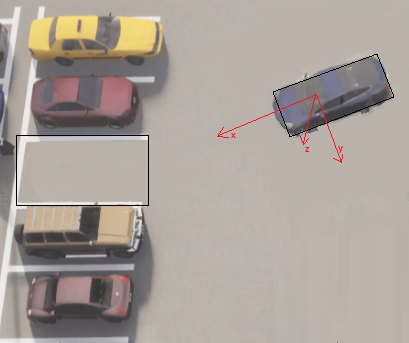
\includegraphics[width=\textwidth]{img/distances_ubi_11}\label {fig:distances11}
    \end{subfigure}
    \begin{subfigure}{0.4\textwidth}
        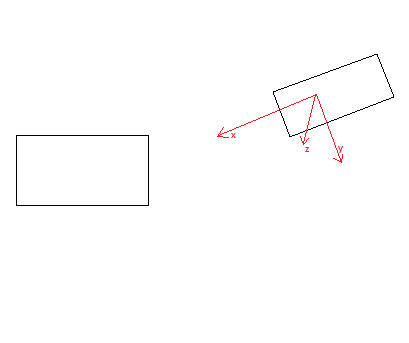
\includegraphics[width=\textwidth]{img/distances_ubi_12}\label {fig:distances12}
    \end{subfigure}
    \caption{Origen del sistema de coordenadas.}
    \label{fig:coord}
\end{figure}
\clearpage

\subsection{Puntos de referencia}
Para representar la posición del vehículo con respecto al espacio de estacionamiento, se establecerán cuatro puntos de referencia:
\begin{itemize}
    \item El punto $1$ se define como la esquina superior izquierda del espacio de estacionamiento.
    \item El punto $2$ se define como la esquina superior derecha del espacio de estacionamiento.
    \item El punto $3$ se define como la esquina inferior izquierda del espacio de estacionamiento.
    \item El punto $4$ se define como la esquina inferior derecha del espacio de estacionamiento.
\end{itemize}
\begin{figure}[!ht]
    \centering
    \begin{subfigure}{0.4\textwidth}
        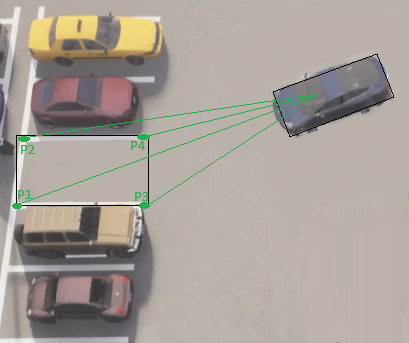
\includegraphics[width=\textwidth]{img/distances_ubi_21}\label {fig:distances21}
    \end{subfigure}
    \begin{subfigure}{0.4\textwidth}
        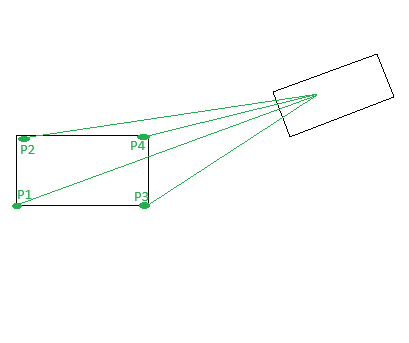
\includegraphics[width=\textwidth]{img/distances_ubi_22}\label {fig:distances22}
    \end{subfigure}
    \caption{Puntos de referencia.}
    \label{fig:coord2}
\end{figure}
\clearpage

\subsection{Coordenadas cilíndricas}
\noindent
Las coordenadas cilíndricas se definen como $(\rho, \theta, z)$, donde:
\begin{itemize}
    \item $\rho$ es la distancia entre el vehículo y un punto de referencia en el espacio de estacionamiento.
    \item $\theta$ es el ángulo de orientación del vehículo con respecto a un punto de referencia en el espacio de estacionamiento.
    \item $z$ es la altura de la cámara con respecto al suelo.
\end{itemize}
\begin{figure}[!ht]
    \centering
    \begin{subfigure}{0.4\textwidth}
        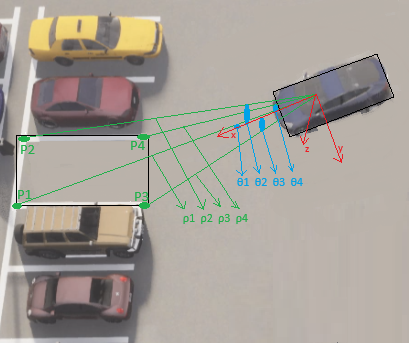
\includegraphics[width=\textwidth]{img/distances_ubi_31}\label {fig:distances31}
    \end{subfigure}
    \begin{subfigure}{0.4\textwidth}
        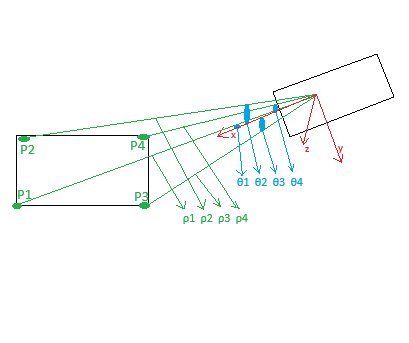
\includegraphics[width=\textwidth]{img/distances_ubi_32}\label {fig:distances32}
    \end{subfigure}
    \caption{Sistema de coordenadas cilíndricas.}
    \label{fig:coord3}
\end{figure}

\subsection{Posición relativa}
La posición relativa del vehículo con respecto al espacio de estacionamiento se representará mediante los 4 vectores de coordenadas cilíndricas:\\
\begin{center}
    $(\rho_1, \theta_1, z)$ , $(\rho_2, \theta_2, z)$ , $(\rho_3, \theta_3, z)$ , $(\rho_4, \theta_4, z)$ \\

\end{center}




